\newcommand{\ComparisonBar}[6]{%
  \pgfmathsetmacro{\ratepos}{4.12+0.183*#3}%
  \node[anchor=west] at (0,#1) {#2};
  \fill[#5] (4.12,#1-0.15) rectangle (\ratepos,#1+0.15);
  \node[anchor=west,xshift=2pt,fill=white,inner sep=1pt] at (\ratepos,#1)
    {\pgfmathprintnumber[fixed,precision=1,fixed zerofill]{#3}};
  \node[anchor=east,inner xsep=0pt] at (10.68,#1) {#4};
  \node[anchor=west,inner xsep=0pt] at (11.38,#1) {#6};%
}

\newcommand{\LibraryComparison}[1]{%
  \begingroup
  \input{generated/comparison-#1.tex}
  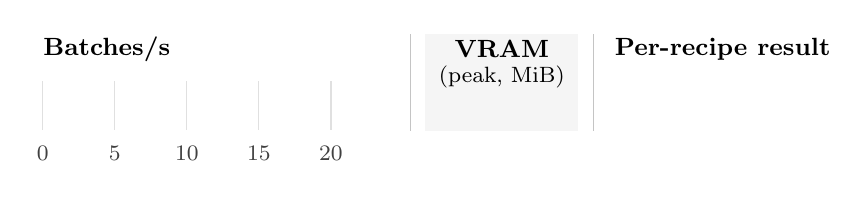
\begin{tikzpicture}[x=1cm,y=0.68cm,font=\small]
  \fill[black!4] (8.98,-0.44) rectangle (10.92,\ComparisonTopRow+1.37);
  \foreach \boundary in {8.79,11.11} {
    \draw[black!23] (\boundary,-0.44) -- (\boundary,\ComparisonTopRow+1.37);
  }
  \node[anchor=west,inner xsep=0pt,font=\small\bfseries] at (4.12,\ComparisonTopRow+1.08) {Batches/s};
  \node[anchor=center,inner sep=0pt,font=\small\bfseries] at (9.95,\ComparisonTopRow+1.08) {VRAM};
  \node[anchor=center,inner sep=0pt,font=\footnotesize] at (9.95,\ComparisonTopRow+0.57) {(peak, MiB)};
  \node[anchor=west,inner xsep=0pt,font=\small\bfseries] at (11.38,\ComparisonTopRow+1.08) {Per-recipe result};
  \foreach \tick in {0,5,10,15,20} {
    \pgfmathsetmacro{\pos}{4.12+0.183*\tick}
    \draw[black!12] (\pos,-0.43) -- (\pos,\ComparisonTopRow+0.49);
    \node[anchor=north,font=\footnotesize,text=black!75] at (\pos,-0.54) {\tick};
  }
  \ComparisonRows
  \end{tikzpicture}
  \endgroup
}

\newcommand{\ComparisonRecipeList}[1]{%
  \begingroup
  \input{generated/comparison-#1.tex}%
  \ComparisonRecipes
  \endgroup
}
